\documentclass[14pt,aspectratio=169,hyperref={pdftex,unicode},xcolor=dvipsnames]{beamer}
\usepackage[english,russian]{babel}
\usepackage[utf8x]{inputenc}
\usepackage[T2A]{fontenc}
\usepackage{cmap}
\usepackage{paratype}
% \usepackage{minted} % для примеров кода (требует параметра -shell-escape)

\usetheme{metropolis}
\usefonttheme[]{professionalfonts}  % запрещаем beamer'у перезаписывать мат. шрифты
\metroset{numbering=fraction}
\metroset{subsectionpage=progressbar}

\setbeamercolor{frametitle}{fg=black}
\setbeamertemplate{frametitle}
{
 \vspace{3mm}\insertframetitle\par
}
\setbeamertemplate{title separator}{}
\setbeamertemplate{footnote separator}{}


\usebackgroundtemplate{
\includegraphics[width=\paperwidth,height=\paperheight]{./common/background_white.jpg}}

\logo{\vspace{-1.2cm}
\includegraphics[width=6mm]{./common/short-v.pdf}\hspace*{1.08\textwidth}}

\institute
{
  \begin{columns}
    \begin{column}{1.5cm}
    
\includegraphics[height=15mm,keepaspectratio]{./common/math-cs.pdf}
    \end{column}
    \begin{column}{4cm}
          Факультет математики и компьютерных наук СПбГУ
    \end{column}
  \end{columns}
}


\begin{document}

\begin{frame}[plain]
  \begin{center}
    \textbf{Андрей Можаев}

    {\Large\textbf{Разработка метода построения упрощенной динамической модели для задачи оптимального управления микроклиматом помещения}}

    Выпускная квалификационная работа

    {\small Научный руководитель: Юрий Рассадин}

%    ДАТА ЗАЩИТЫ
  \end{center}


  \begin{columns}
    \begin{column}{1cm}
    
\includegraphics[height=15mm,keepaspectratio]{./common/math-cs.pdf}
    \end{column}
    \begin{column}{10cm}
      \small
          Факультет математики и~компьютерных наук СПбГУ\\
          Программа <<Современное программирование>>
    \end{column}
  \end{columns}
\end{frame}



\begin{frame}
\frametitle{Введение в предметную область}

\begin{itemize}
\item На управление микроклиматом (системы отопления, вентиляции и кондиционирования) в зданиях общего пользования уходит до 70\% всей потребляемой энергии.
\item Для повышения качества регулирования необходимы модели предсказания температуры воздуха в помещениях
\end{itemize}

\end{frame}



\begin{frame}
\frametitle{Введение в предметную область}

\begin{itemize}
\item Одним из факторов, влияющих на предсказания, является расположение датчика
\item Цель найти оптимальное расположение, в котором предсказания будут наиболее точными
\item Будем решать эту задачу численно
\item Аналогичные подходы численного моделирования применяются при проектировании систем вентиляции
\end{itemize}

\end{frame}



\begin{frame}
\frametitle{Постановка задачи}
\begin{enumerate}
\item Построить модель помещения методами вычислительной гидрогазодинамики (CFD), промоделировать некоторый промежуток времени с хорошей точностью
\item Анализируя накопленный массив данных, найти оптимальную точку для размещения датчика
\end{enumerate}
\end{frame}



\begin{frame}{Моделирование помещения}
\small
\begin{itemize}
\item ПО для моделирования - COMSOL
\item Помещение для моделирования - "проект демонстрационного стенда Умного дома" (комната 10x6x3 с окном и внутренней стеной)
\item Температура окружающей среды взята из датасета с реальными температурами в августе 2020 года
\item Также промоделирована солнечная радиация
\end{itemize}

\begin{center}

\includegraphics[width=8cm]{images/logo_comsol.png}
\end{center}

\end{frame}



\begin{frame} \begin{center}
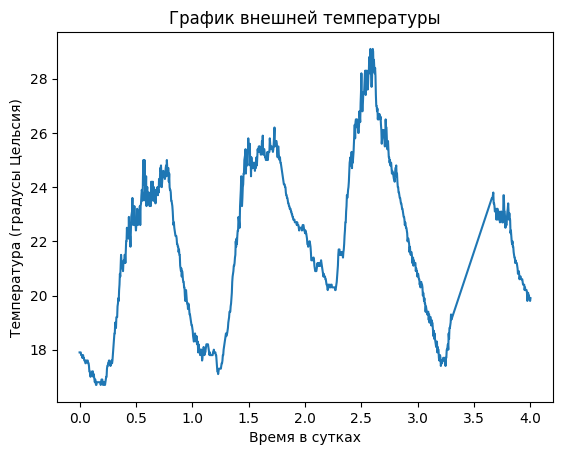
\includegraphics[width=11cm]{images/temperature_plot.png}
\end{center} \end{frame}

\begin{frame} \begin{center}
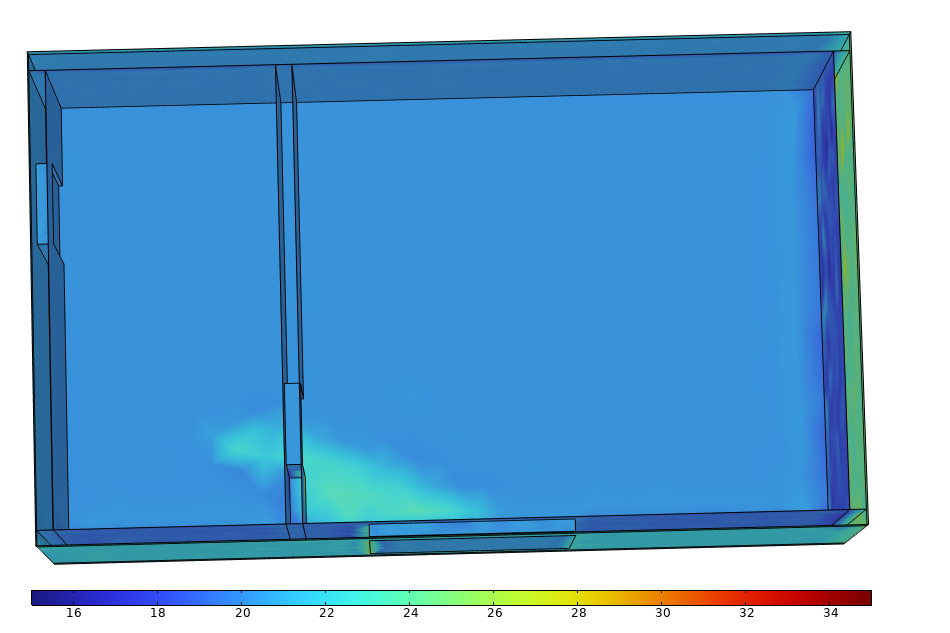
\includegraphics[width=11cm]{images/solar_radiation/solar_1.png}
\end{center} \end{frame}
\begin{frame} \begin{center}
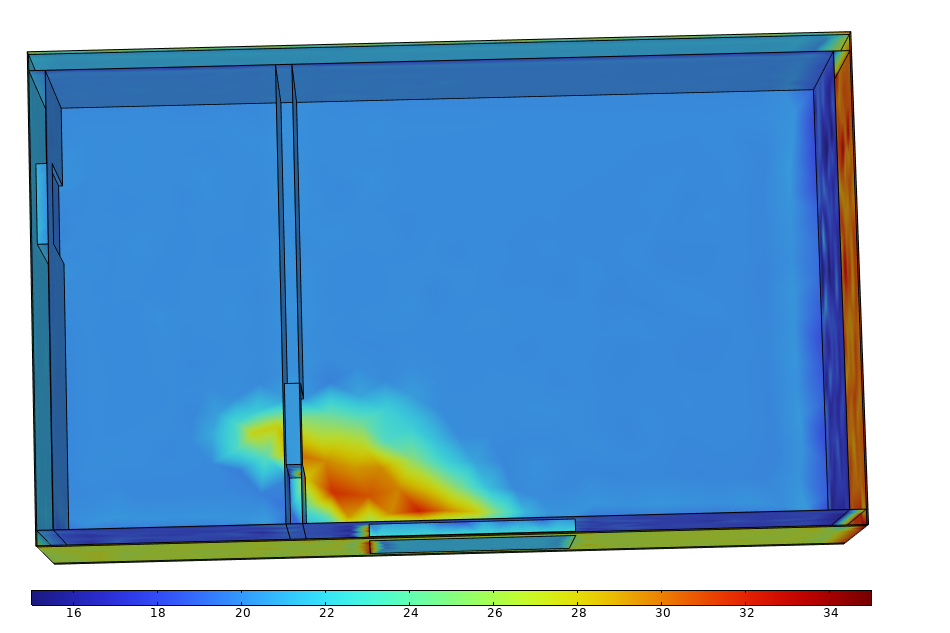
\includegraphics[width=11cm]{images/solar_radiation/solar_2.png}
\end{center} \end{frame}
\begin{frame} \begin{center}
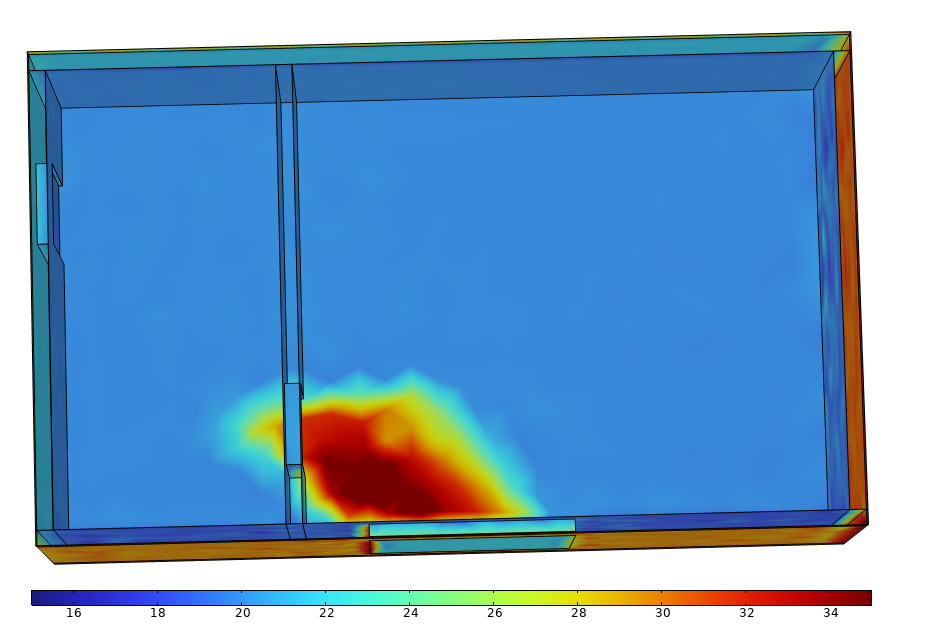
\includegraphics[width=11cm]{images/solar_radiation/solar_3.png}
\end{center} \end{frame}
\begin{frame} \begin{center}
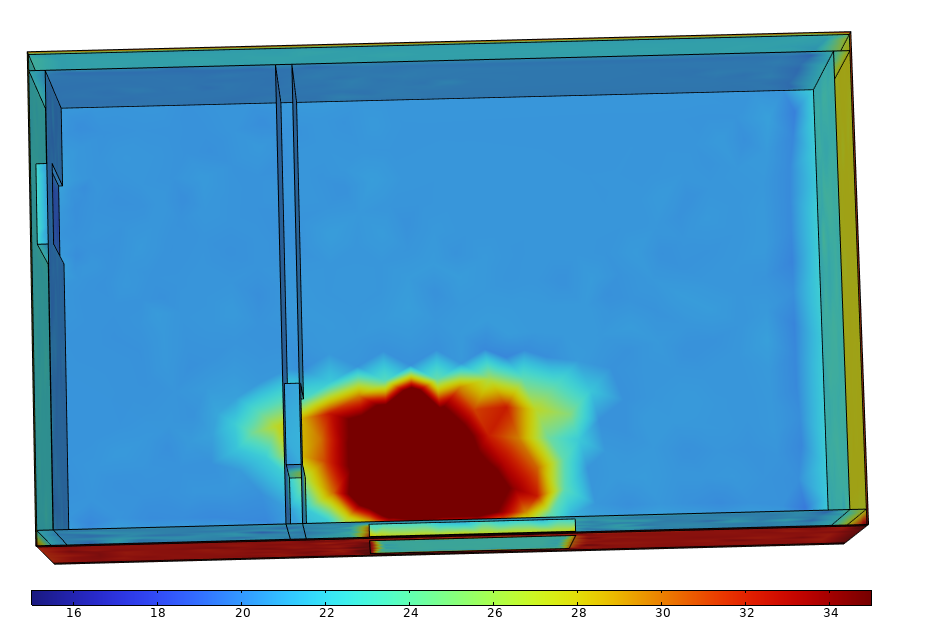
\includegraphics[width=11cm]{images/solar_radiation/solar_4.png}
\end{center} \end{frame}
\begin{frame} \begin{center}
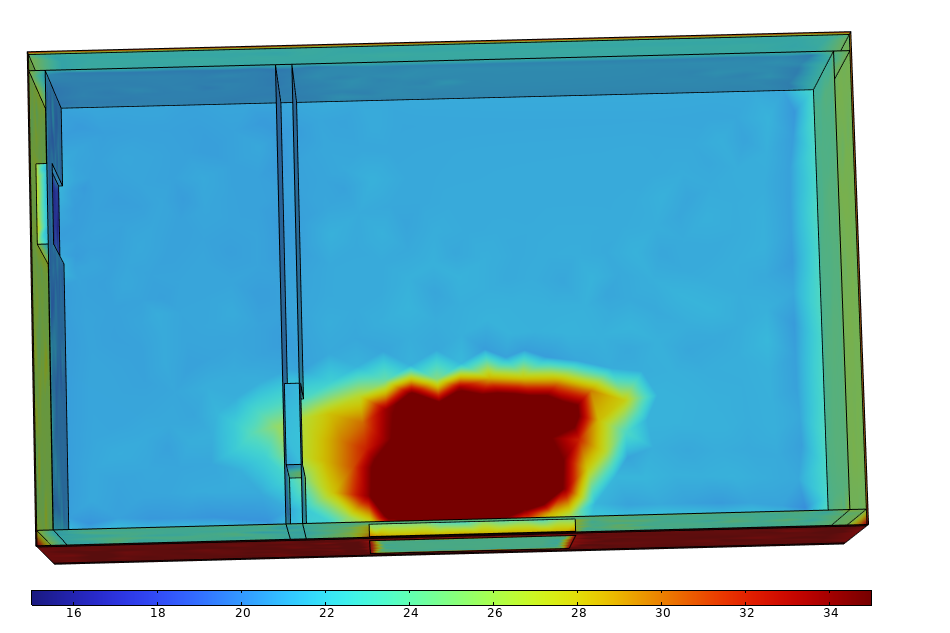
\includegraphics[width=11cm]{images/solar_radiation/solar_5.png}
\end{center} \end{frame}
\begin{frame} \begin{center}
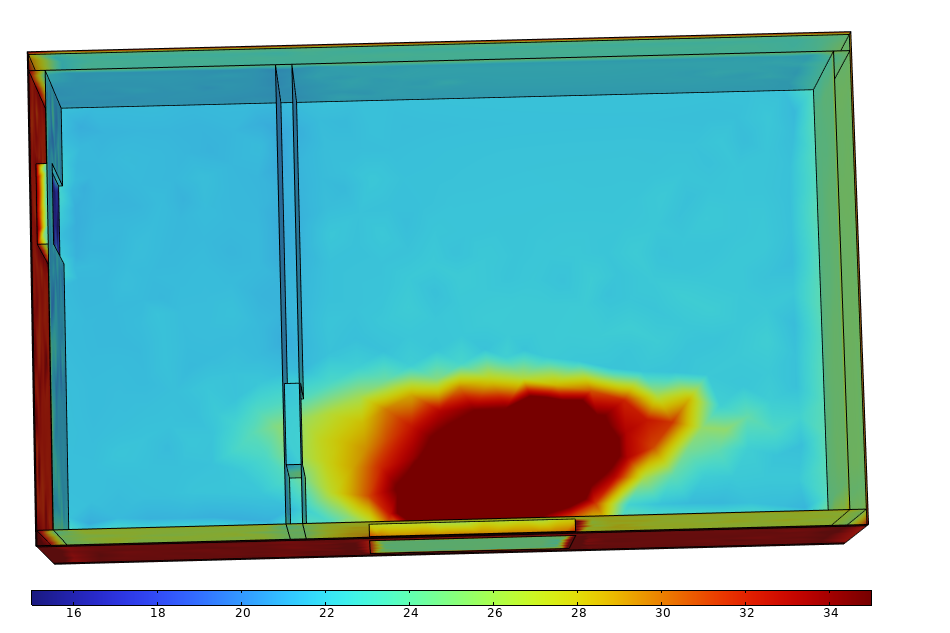
\includegraphics[width=11cm]{images/solar_radiation/solar_6.png}
\end{center} \end{frame}
\begin{frame} \begin{center}
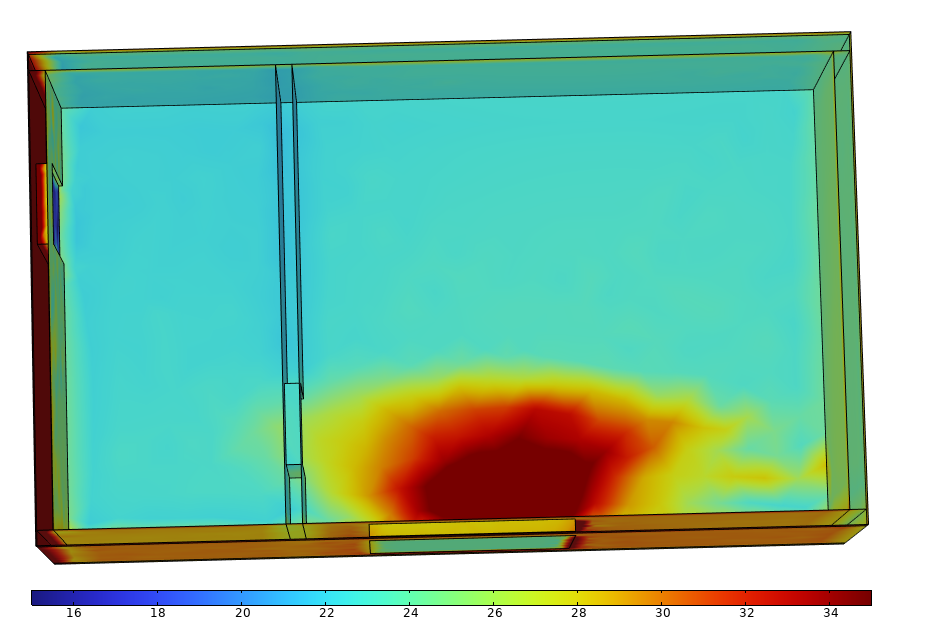
\includegraphics[width=11cm]{images/solar_radiation/solar_7.png}
\end{center} \end{frame}
\begin{frame} \begin{center}
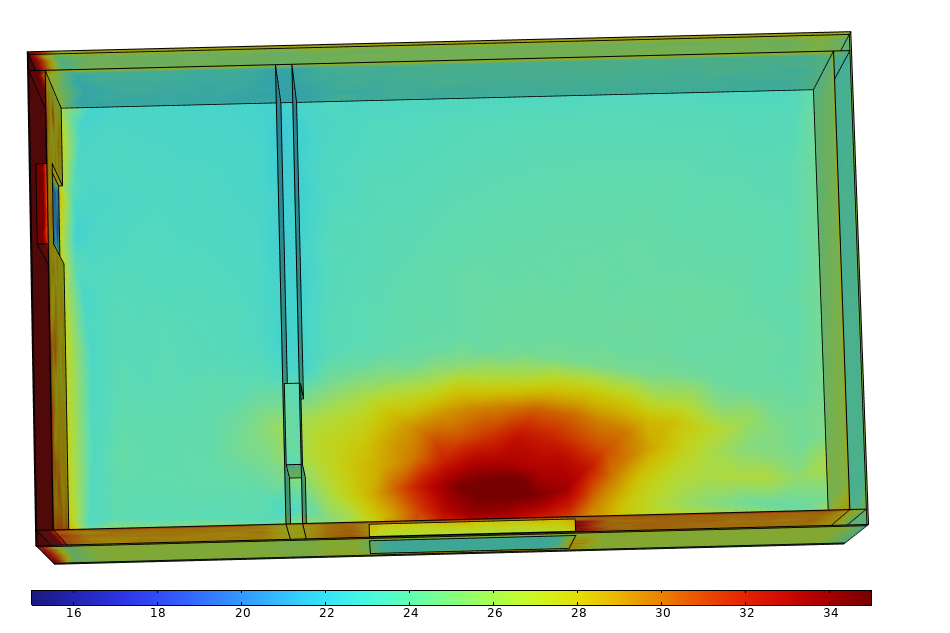
\includegraphics[width=11cm]{images/solar_radiation/solar_8.png}
\end{center} \end{frame}



\begin{frame}{Поиск оптимального расположения датчика}

\begin{itemize}
\item Построение линейной модели для потенциальной точки размещения датчика
\item Сравнение качества предсказания с остальными точками
\end{itemize}

\end{frame}



\begin{frame}

\begin{center}
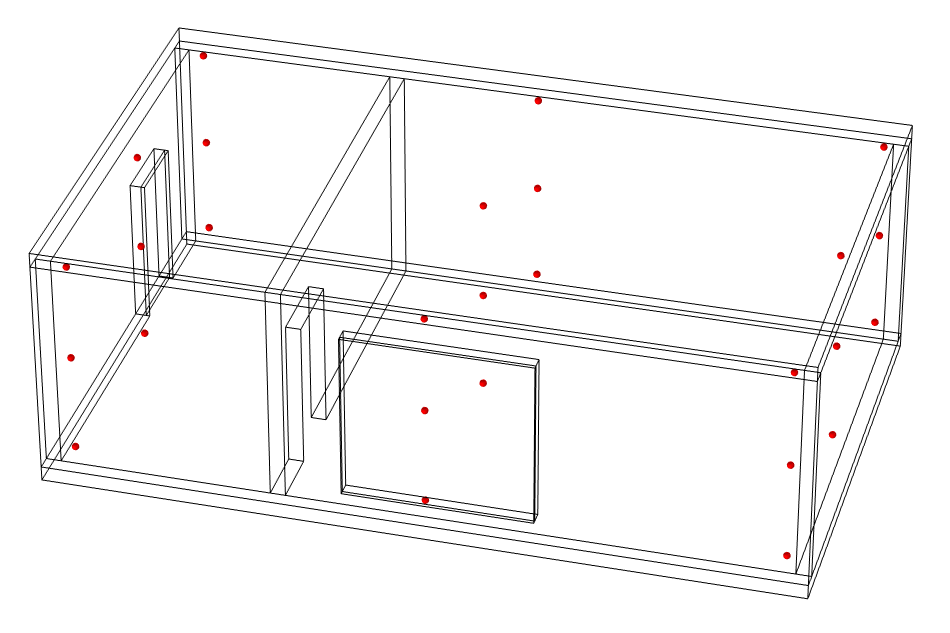
\includegraphics[width=11cm]{images/interesting_points.png}
\end{center}

\end{frame}



\begin{frame}{Результат моделирования}
\centering
\begin{table}[]
\begin{tabular}{c|c|c|c|c|c}
\textbf{Time (s)} & \textbf{Point 1} & \textbf{Point 2} & ... & \textbf{Point 27} & \textbf{Ambient} \\ \hline
0                 & 20.0             & 19.4             &     & 20.8              & 17.9             \\
300               & 19.9             & 19.4             &     & 20.7              & 17.9             \\
600               & 19.9             & 19.4             &     & 20.6              & 17.9             \\
...               &                  &                  &     &                   &                  \\
345600            & 21.2             & 21.5             &     & 20.8              & 19.9            
\end{tabular}
\end{table}

\end{frame}



\begin{frame}{Критерий оптимальности}

\begin{itemize}
\item Первым делом определим критерий оптимальности точки
\item Частоты колебаний внешней и внутренней температур совпадают, но существует сдвиг по фазе \footnote{Пащенко А.Ф., Рассадин Ю.М. Оценка взаимосвязи параметров микроклимата с учетом тепловой инерции внешних стен здания / Труды 15-й Международной конференции "Управление развитием крупномасштабных систем" (MLSD’2022). М.: ИПУ РАН, 2022. С. 1216-1224.}
\end{itemize}

\end{frame}



\begin{frame} \begin{center}
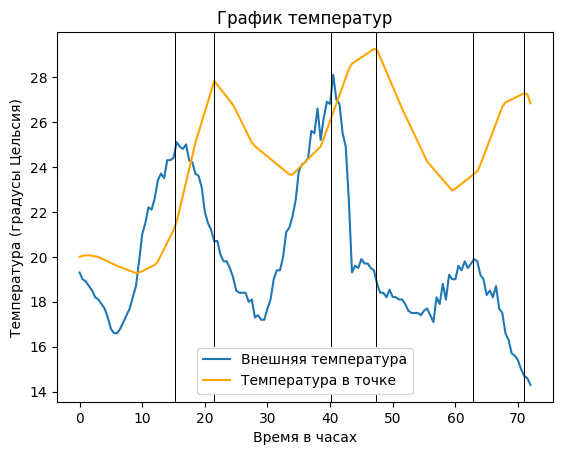
\includegraphics[width=11cm]{images/indent.png}
\end{center} \end{frame}
\begin{frame} \begin{center}
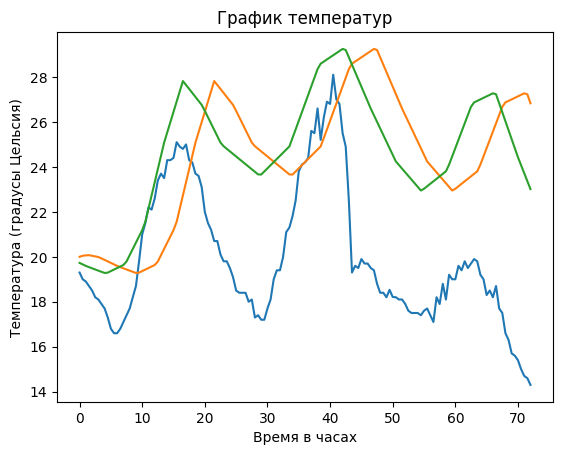
\includegraphics[width=11cm]{images/indent_2.png}
\end{center} \end{frame}



\begin{frame}{Критерий оптимальности}

\begin{itemize}
\item Находить размер сдвига будем с помощью критерия корреляции Пирсона для временных рядов. Для каждой пространственной точки этот сдвиг может быть разным
\item Затем для сдвинутого ряда температур находим коэффициенты линейной регрессии
\item Точка с наибольшим коэффициентом детерминации $R^2$ будет оптимальной
\end{itemize}

\end{frame}



\begin{frame} \begin{center}
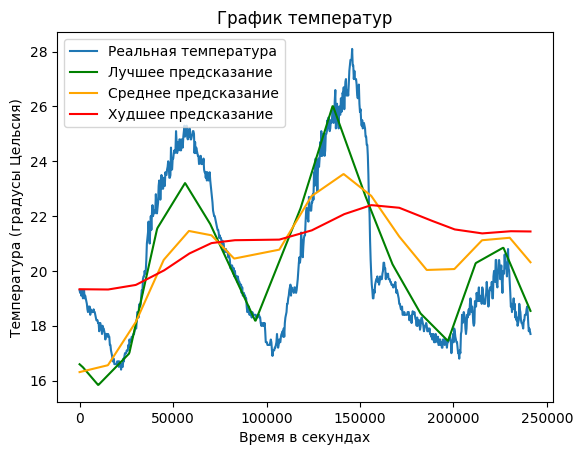
\includegraphics[width=11cm]{images/result.png}
\end{center} \end{frame}

\begin{frame} \begin{center}
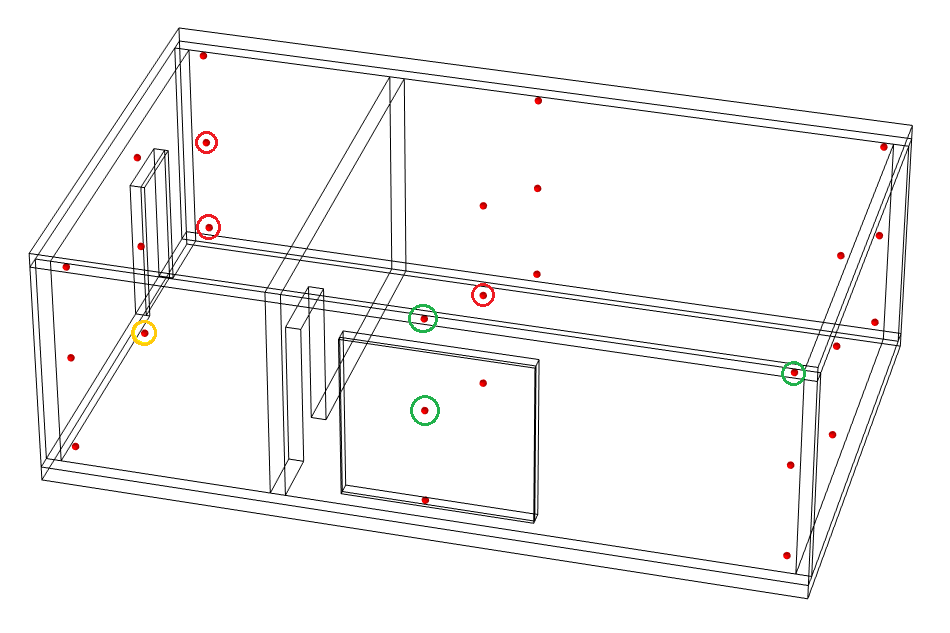
\includegraphics[width=11cm]{images/interesting_points_result.png}
\end{center} \end{frame}



\begin{frame}
\frametitle{Результаты работы}

\begin{enumerate}
\item Промоделированно помещение с реальной внешней температурой
\item Разработан алгоритм нахождения оптимальной точки расположения датчика
\end{enumerate}

\vspace{5mm}\hrule\vspace{5mm}

\begin{center}
Андрей Можаев, email: mozhay2000@gmail.com\\
https://github.com/mozhayka/microclimate
\end{center}

\end{frame}



\end{document}
